\documentclass{article}
\usepackage[utf8]{inputenc}
\usepackage[margin=1in,left=1.5in,includefoot]{geometry}
\usepackage{booktabs}
\usepackage{graphicx}
\usepackage{hyperref}
\usepackage{wrapfig}
\usepackage{amsmath}
\usepackage{amssymb}

% Header & Footer Stuff

\usepackage{fancyhdr}
\pagestyle{fancy}
\lhead{Visión por Computador Aplicada}
\rhead{614G030332425}
% \fancyfoot{}
% \lfoot{Pablo Chantada Saborido \& José Romero Conde}
% \fancyfoot[R]{}

% The Main Document
\begin{document}
	\begin{center}
		\LARGE\bfseries PRÁCTICA II\\
		\small Pablo Chantada Saborido \& José Romero Conde
		\line(1,0){430}
	\end{center}
	
\vspace*{380pt}
	
\begin{figure}[h]
	\centering
	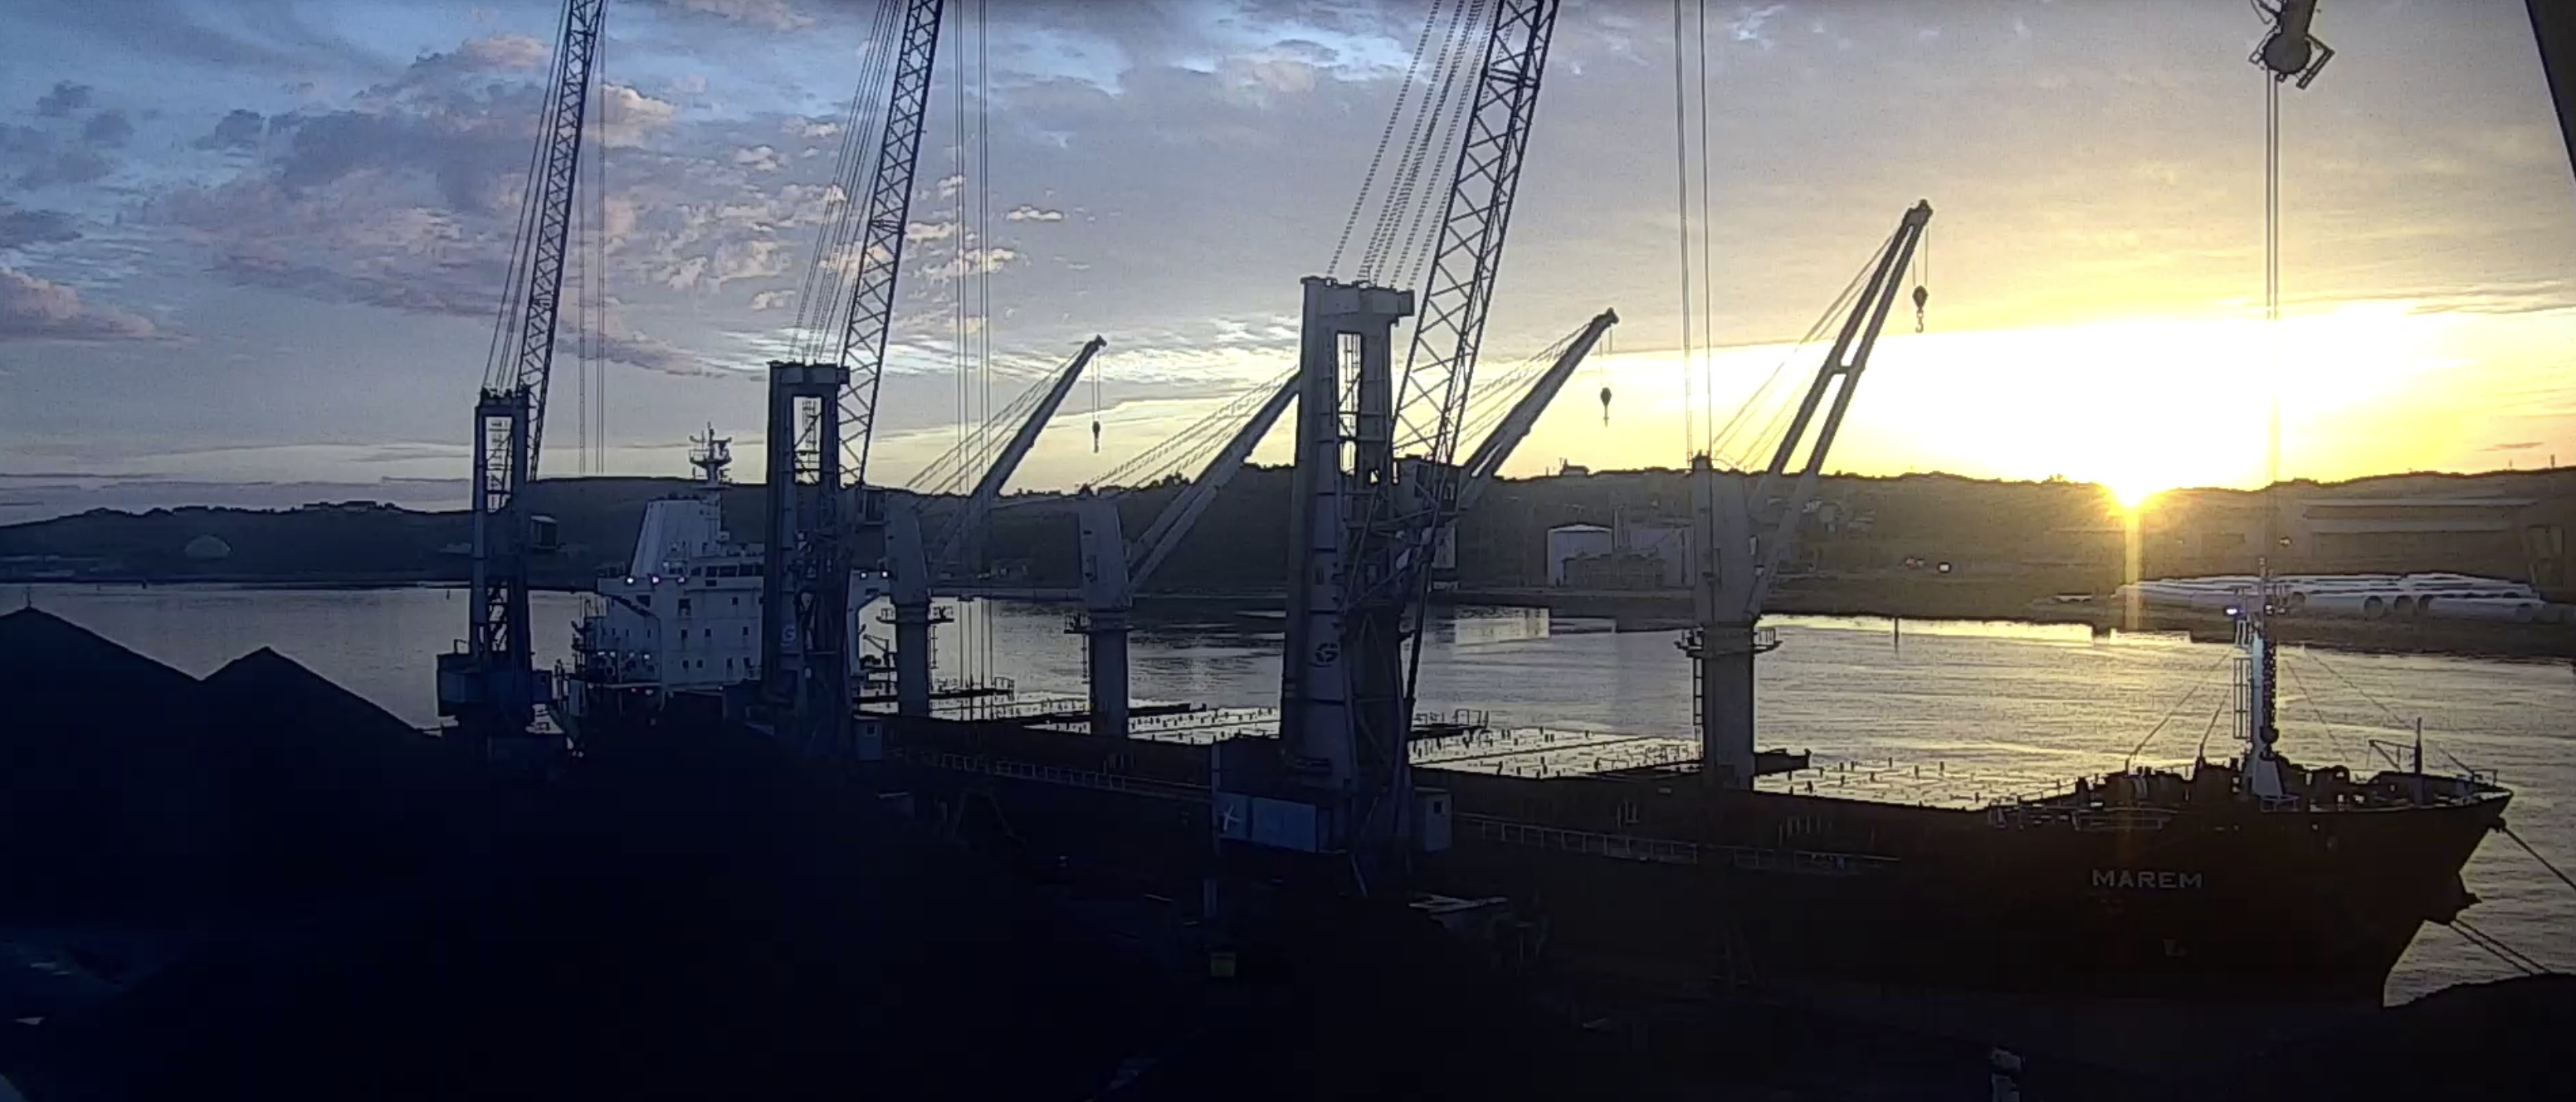
\includegraphics[width=0.7\linewidth]{portada}
	\label{fig:portada}
\end{figure}
	
\thispagestyle{empty}
	
\newpage
	
	
	
\section*{Introducción}

\section*{Clasificación Ship/No-ship}
\subsection*{Modelo base}

Describimos ahora nuestro modelo baseline, que nos valió para iterar y comparar resultados. El modelo se compone de los siguientes elementos:

\begin{itemize}
	\item  \textbf{\href{https://arxiv.org/pdf/1905.11946}{EfficientNet.}} La usamos como CNN de partida. Originalmente pensamos que tenía como requirimiento que las imágenes sean de tamaño $(244,244,3)$, para ello implementamos un recortador automático de \emph{el cuadrado más grande} que llamamos desde los \texttt{DataLoader} de entrenamiento y test. Mas tarde nos dimos cuenta que la red era realmente capaz de procesar iménes de cualquier tamaño porque tiene al final de todo un \texttt{Global Pooling}. No obstante, como de cualquier forma los \emph{mini-batches} tenían que ser todos del mismo tamaño decidimos quedarnos con la idea de recortar las imágenes de la forma mencionada.
	\item \textbf{Aumento de datos.} El aumento de datos en esta fase esencialmente consta de dos partes, por un lado, las transformaciones de \texttt{torchvision.transforms} y por otro imágenes recortadas a mano. Con respecto a lo primero, nosotros usamos: volteos horizontales, fluctuaciones leves en el color, también leves trasnformaciones afines y conversión a blanco y negro con baja probabilidad. El segundo punto es que hemos recortado manualmente las imagenes de barcos de forma que queden cerntrados y sin fondo que estorbe, se han añadido estas images al conjunto de datos cuando se especificaba aumento de datos. De esta forma conseguimos dos cosas distintas: 
	\begin{itemize}
		\item Representar más variaciones que las presentes en el conjunto de entrenamiento, con la esperanza de que si sí ocurriesen en test, estaríamos preparados.
		\item Representar con menos ruído adicional lo que sí queremos aprender. Porque aunque es beneficioso para la red someterse a mucha variación, también dificulta el entrenamiento (es un problema más difícil).
\end{itemize}
	\item Un \textbf{MLP} de tres capas, sobre la salida de la red. La salida de la última capa \texttt{nn.Softmax()} tiene 2 o 3 neuronas según si se quería clasificar en \{no barco, barco\} o en \{no barco, barco no amarrado, barco amarrado\}. 
\end{itemize}

\subsection*{Entrenamiento y evaluación}

El entrenamiento fue díficil y además somos inexpertos pero hemos identificado algunos problemas para los que hemos encontrado solución. Aquí se presentan:
\begin{itemize}
	\item \textbf{Datos no balanceados.} Observamos que la red, \emph{hackeando} nuestras métricas decidía que todas las imágenes eran barcos (147 contra 88). Afrontamos esto alterando la probailidad de ocurrencia de las clases de forma que si antes, al escoger una imagen de \texttt{DataLoader}, $p(X=barco) = \frac{147}{147+88}$ ahora $p(X = barco) = 0.5$. Para ello usamos la utilidad \texttt{WeightedRandomSampler} de torch.
	\item \textbf{Capacidad del modelo.} Originalmente usamos la EfficientNet-B0, pero viendo malos resultados decidimos cambiar a la EfficientNet-B3, que es un poco más grande pero precisamente como explican en el artículo, sigue siendo muy eficiente.
	\item \textbf{Mínimos locales.} Probablemente si solucionásemos este problema de forma total estaríamos cerca de ganar un Nobel, naturalmente no lo hemos hecho. Pero para aliviar las consecuencias implementamos un \texttt{learning\_rate} que, con una cierta paciencia, mediaba su valor. \footnote{Esta paciencia mencionada y la del \emph{earlystopping} pueden ambas ser ajustadas como \emph{flags} en nuestro script.}
	\item \textbf{Sobreajuste y generalización.} Para cercionarnos de que la red aprendía correctamente, añadimos una penalización de la norma eucídea en la función de perdida, es decir, regularización Tikhonov.
\end{itemize}


\begin{wrapfigure}{l}{0.3\textwidth}
	\includegraphics[width=1\linewidth]{cmEj1} 
	\label{fig:cmEj1}
	%\caption{Matriz de confusión para el primer ejercicio}
\end{wrapfigure}


Otras consideraciones sobre el entrenamiento que consideramos menos profundas y más ordinarias son: como optimizador hemos usado \href{https://arxiv.org/pdf/1711.05101}{AdamW} con un \texttt{learning\_rate} de $10^{-4}$. Usamos un \texttt{batch\_size} de 16, que aunque es relativamente pequeño, no mucho más pueden hacer nuestros portátiles. 

Con respecto a los resultados obtenidos en esta primera iteración, pueden observarse a grandes rasgos en la matriz de confusión de la izquierda, la cual nosotros prudentemente podemos decir que estamos orgullosos porque las predicciones de la red se concentran en las etiquetas verdaderas, fallando en sólo una imagen de 59. Figuras de las curvas de pérdida y precisión en aprendizaje o de las etiquetas predichas por la red para algunas imágenes en concreto pueden encontrarse para este ejercicio y el siguente en el Apéndice al final del documento.


\section*{Clasificación Docked/Undocked}

Nosotros concebimos este ejercicio como una extensión del ejercicio anterior, de esta forma pensamos en reutilizar todas las representaciones aprendidas.
\begin{itemize}
	\item Cuando se especifica \texttt{pretrained=True}, nuestra red no toma los pesos de Imagenet, sino del ejercicio anterior. De esta forma ya tiene mucho aprendido y el proceso de optimización será más sencillo.
	\item Como ahora la cabeza de la red tiene 3 neuronas pero antes tenía 2, en vez de inicializar aleatoriamente las tres neuronas \footnote{Como nuestro MLP tiene una única capa, cada neurona es un único vector del tamaño de salida de la red (1536 en el caso de la EfficientNet-B3), y esto significa que estamos asumiendo que el problema es linealmente separable en el espacio $\mathbb{R}^{1536}$. Esto me parece interesante chanti pero borralo si quieres}, dos se copian y sólo una se inicializa aleatoriamente. De nuevo, de esta forma tiene menos trabajo por delante.
\end{itemize}

\section*{Resultados}

\begin{wrapfigure}{l}{0.3\textwidth}
	\includegraphics[width=1\linewidth]{cmEj2} 
	\label{fig:cmEj2}
	%\caption{Matriz de confusión para el segundo ejercicio}
\end{wrapfigure}

Aunque a priori parece que son peores resultados que en el ejercicio 1, queremos señalar las siguientes observaciones:

\begin{itemize}
	\item Ahora el problema original (barco contra no barco) está totalmente resuelto (no barco tiene la etiqueta de 0). A esto le encontramos la siguiente intuición: que la red se esfuerce en un problema más complejo hace que sea más capaz de resolver el problema sencillo.
	\item Las diferencias entre las clases atracado contra no atracado son realmente sutiles [poner foto] y a un humano (nosotros probamos con amigos) que no ha sido \emph{entrenado} con las etiquetas también le puede resultar complejo resolver.
	\item No obstante en general podríamos decir que aunque la clasificación no es perfecta por lo menos es bastante diagonal.
\end{itemize}

\subsection*{Evaluación de modelos}

\subsection*{Análisis de resultados}

\section*{Conclusión}


\section*{Apéndice}

\begin{figure}[h]
	\centering
	\includegraphics[width=0.9\linewidth]{lossEj1}
	\label{fig:lossEj1}
	\caption{Loss y Accuracy para el primer ejercicio}
\end{figure}

\begin{figure}[h]
	\centering
	\includegraphics[width=0.8\linewidth]{imagenesEj1}
	\label{fig:imagenesEj1}
	\caption{Imágenes con su etiqueta correcta y el vector SoftMax predicha por la red para el primer ejercicio}
\end{figure}

%\begin{figure}[h]
%	\centering
%	\includegraphics[width=0.5\linewidth]{cmEj2}
%	\label{fig:cmEj2}
%	\caption{Matriz de confusión para el segundo ejercicio}
%\end{figure}

\begin{figure}[h]
	\centering
	\includegraphics[width=0.9\linewidth]{lossEj2}
	\label{fig:lossEj2}
	\caption{Loss y Accuracy para el segundo ejercicio}
\end{figure}

\begin{figure}[h]
	\centering
	\includegraphics[width=0.8\linewidth]{imagenesEj2}
	\label{fig:imagenesEj2}
	\caption{Imágenes con su etiqueta correcta y el vector SoftMax predicha por la red para el segundo ejercicio}
\end{figure}




















\end{document}

